\section{Chile}
\label{sec:chile}



\begin{spice}\label{spice:chile}
\textsc{Chile} \hfill \href{https://powo.science.kew.org/taxon/316944-2}{POWO} \\
\textbf{English:} \textit{chile}. 
\textbf{Arabic:} {\arabicfont{فلفل حار}} \textit{fulful hārr} [hot pepper]. 
\textbf{Chinese:} {\tradchinesefont{辣椒}} \textit{làjiāo} [pungent-pepper]. 
\textbf{Hungarian:} \textit{paprika}; \textit{pirospaprika} [red-pepper]; \textit{fűszerpaprika} [spice-pepper]; \textit{erős-paprika} [strong-pepper]; \textit{csilipaprika} [chili-pepper]; \textit{Cayenne bors} [Cayenne pepper]; \textit{törökbors} [Turkish-pepper] (historic).  \\
\noindent{\color{black}\rule[0.5ex]{\linewidth}{.5pt}}
\begin{tabular}{@{}p{0.25\linewidth}@{}p{0.75\linewidth}@{}}
Plant species: & \taxonn{Capsicum annuum}{L.}; \textit{\taxonn{Capsicum frutescens}{L.}; \taxonn{Capsicum chinense}{Jacq.}; et al.} \\
Family: & \textit{Solanaceae} \\
part used: & fruit \\
Region of origin: & Central America \\
Cultivated in: & Ethiopia; India; Kenya; Mexico; Nigeria; Pakistan; Tanzania; etc. \\
Color: & red and green in many shades \\
\end{tabular}
\end{spice}

% \begin{figure}[!ht]
% 	\vspace{-4ex}
% 	\centering
% 	\subfloat[\centering a]{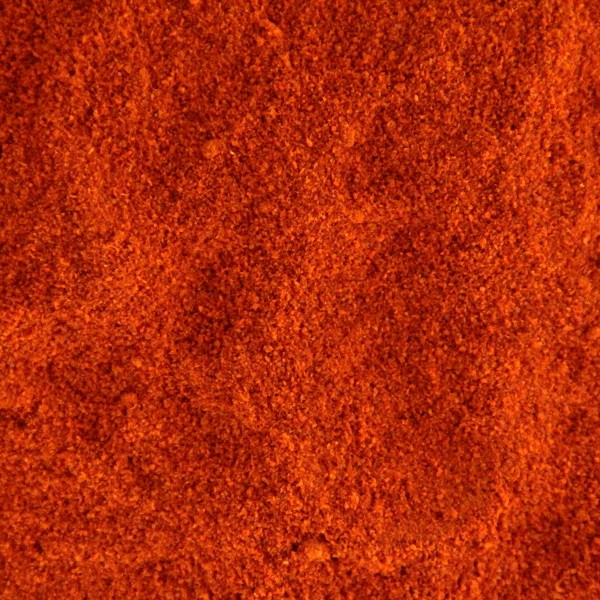
\includegraphics[width=0.3\linewidth]{imgs/spices/chile-1.jpg}}
% % 	\hfill
% % 	\subfloat[\centering b]{\includegraphics[width=0.3\linewidth]{imgs/spices/chile-2.jpg}}
% % 	\hfill
% % 	\subfloat[\centering c]{\includegraphics[width=0.3\linewidth]{imgs/spices/chile-3.jpg}}
% 	\caption{Chile \taxon{}.}
% 	\label{fig:chile_imgs}
% \end{figure}

\begin{wrapfigure}{R}{0.33\textwidth}
	\vspace{-\baselineskip}
	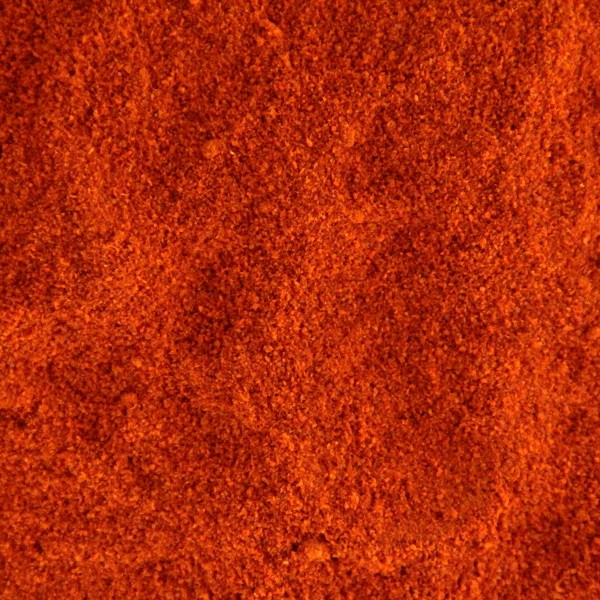
\includegraphics[width=0.33\textwidth]{imgs/spices/chile-1.jpg}
	\caption{Chili powder (\taxon{Capsicum annuum}, et al.).}
	\label{fig:chile}
\end{wrapfigure}

Chile, chili, or chilli, is the pod-like fruit of various species of \textit{Capsicums}, most prominently \taxon{Capsicum annuum}, \taxon{C. frutescens} their countless \glspl{cultivar}, but other species are used as a spice as well. The chili pepper---as it is conventionally called---is used both fresh and dry, and it is the most recognizable spice of our time. Since its rapid diffusion across the globe with the \gls{Columbian}, it dominates many of the world's dishes and cuisines with its heat and aromatic flavour. 
% Many books have been written about the success of chili, and I do not want to enumerate the words 

\subsection{The Botany, Origins, and Cultivation of Chile}

\subsection{The History of Chile}

The history of the chili is very well documented, and its diffusion is a well known historical phenomenon after the initial European contact. In his writings Columbus only mentions \textit{ají}, and its extreme heat, but the Europeans were so set on finding spices that was already known to them, that the excitement of this new spice---the chile pepper---evaded them at first. The Spanish had no idea that chile will soon take over the world by storm. Ají, the Taíno word for chile is still used today in the Caribbean. In January 15 of 1942, he wrote in his personal log about the island of Hispaniola: ``There is also plenty of ají, which is their pepper, which is more valuable than [black] pepper, and all the people eat nothing else, it being very wholesome. Fifty caravels might be annually loaded with it.'' \autocites[11]{turner_spice_2004}. For the story, I recommend \textcite{wright_medieval_2007}'s \textit{The Medieval Spice Trade and the Diffusion of the Chile}, and for the history of chile in a Chinese context, there is a great new monograph by \textcite[]{dott_chile_2020}.

% Dalby 150:
% One of the things that Columbus particularly wished to do was to find pepper - not quite the most expensive spice in medieval Europe, but the one in most demand. He and his followers came to call the capsicum species 'pepper of the Indies'. 




% Turner 11:
% Peter Martyr, the Italian humanist at the Spanish court, noted that five grains of the new plant brought back by Columbus were hotter and more flavorful than twenty grains of Malabar pepper. Columbus himself was taken aback by its heat, reporting to the king and queen (like many an unwary newcomer since) that he found Caribbean food “extremely hot.” The natives seemed to put their pepper into everything.
%  Not even such a dreamer as Columbus could have foreseen the future success of his aji: It was, of course, the chili, and it was growing wild all over Spain’s new possessions. Within decades the plant had spread so rapidly around the world that Europeans traveling in Asia expressed confusion as to its origin,

\subsection{The Names of Chile}

\subsubsection{English}

\begin{etymology}\label{ety:chile}
English \textit{chilli}, XVII Ee 1660 Et 1604 Mw
< Spanish \textit{chile} `id.'
< Classical Nahuatl \textit{chīlli} `id.'\footnote{}
\end{etymology}

\begin{etymology}\label{ety:paprika}
\textbf{English} \textit{paprika}
< \textbf{Hungarian} \textit{paprika}, diminutive?
< \textbf{Serbian-Croatian-Bosnian} \textit{paprika} `little pepper', (papar+ika) papar = pepper; -ika = Suffix appended to words to create a feminine noun, usually denoting a plant.
< \textbf{Slavic} {*pьpьrь} \textit{*pĭpĭrĭ }
< \textbf{Latin} \textit{piper}
< \textbf{Ancient Greek} {πέπερι} \textit{péperi}
< \textbf{Pahlavi} \textit{?}
< \textbf{Middle Indo-Aryan} \textit{pipparī}
< \textbf{Sanskrit} \textit{pippalī}\footnote{; }
\end{etymology}

\begin{table}[!ht]
\centering
\begin{tabularx}{\textwidth}{@{}l>{\itshape \small}lL>{\small}l@{}}
\toprule
\textbf{\#} & \multicolumn{1}{l}{\textbf{Species}} & \multicolumn{1}{l}{\textbf{Name}} & \multicolumn{1}{l}{\textbf{Source}} \\
\midrule
1	& Capsicum annuum	& paprika	& \textcite{van_wyk_culinary_2014} \\
2	& Capsicum annuum Grossum	& bell-pepper	& \textcite{oed} \\
3	& Capsicum annuum Grossum	& green pepper	& \textcite{van_wyk_culinary_2014} \\
4	& Capsicum annuum Longum	& paprika pepper	& \textcite{oed} \\
5	& Capsicum annuum Longum	& sweet pepper	& \textcite{oed} \\
6	& Capsicum annuum var. glabriusculum	& bird pepper	& \textcite{oed} \\
7	& Capsicum annuum; C. frutescens	& Cayenne pepper	& \textcite{van_wyk_culinary_2014} \\
8	& Capsicum annuum; C. frutescens	& Guinea pepper	& \textcite{oed} \\
9	& Capsicum annuum; C. frutescens	& Indian pepper	& \textcite{oed} \\
10	& Capsicum cerasiforme	& cherry-pepper	& \textcite{oed} \\
11	& Capsicum frutescens	& bird chili	& \textcite{van_wyk_culinary_2014} \\
12	& Capsicum frutescens	& hot pepper	& \textcite{van_wyk_culinary_2014} \\
13	& Capsicum frutescens	& piri piri	& \textcite{van_wyk_culinary_2014} \\
14	& Capsicum frutescens	& Tabasco pepper	& \textcite{van_wyk_culinary_2014} \\
15	& Capsicum spp.	& capsicum	& \textcite{oed} \\
\textbf{16}	& \textbf{Capsicum spp.}	& \textbf{chili}	& \textbf{\textcite{van_wyk_culinary_2014}} \\
17	& Capsicum spp.	& chili pepper	& \textcite{van_wyk_culinary_2014} \\
18	& Capsicum spp.	& pepper	& \textcite{oed} \\
19	& Capsicum spp.	& pod pepper	& \textcite{oed} \\
20	& Capsicum spp.	& red pepper	& \textcite{van_wyk_culinary_2014} \\
\bottomrule
\end{tabularx}
\caption{Various names for chile in English.}
\label{table:names_chile_en}
\end{table}



\subsubsection{Arabic}

\begin{etymology}\label{ety:fulful harr}
\textbf{Arabic} {فلفل حار } \textit{fulful ḥārr} `chili pepper' [hot pepper]\footnote{\textcite{wehr_dictionary_1976}}
\end{etymology}

\begin{table}[!ht]
\centering
\begin{tabularx}{\textwidth}{@{}l>{\itshape \small}lr>{\itshape}lL>{\small}l@{}}
\toprule
\textbf{\#} & \multicolumn{1}{l}{\textbf{Species}} & \multicolumn{1}{l}{\textbf{Name}} & \multicolumn{1}{l}{\textbf{Tr.}} & \multicolumn{1}{l}{\textbf{Gloss}} & \multicolumn{1}{l}{\textbf{Source}} \\
\midrule
1	& Capsicum spp.	& بابريكا	& bābrīkā	& paprika	& \textcite{wikipedia} \\
2	& Capsicum spp.	& فليفلة	& fulayfila	& little pepper	& \textcite{wehr_dictionary_1976} \\
3	& Capsicum spp.	& فلفل أخضر	& fulful akhḍar	& green pepper	& \textcite{wehr_dictionary_1976} \\
4	& Capsicum spp.	& فلفل أحمر	& fulful aḥmar	& red pepper	& \textcite{baalbaki_-mawrid_1995} \\
5	& Capsicum spp.	& فلفل حلو	& fulful ḥulw	& sweet pepper	& \textcite{baalbaki_-mawrid_1995} \\
\textbf{6}	& \textbf{Capsicum spp.}	& \textbf{فلفل حار }	& \textbf{fulful ḥārr}	& \textbf{hot pepper}	& \textbf{\textcite{baalbaki_-mawrid_1995}} \\
7	& Capsicum spp.	& فلفل	& fulful, filfil	& 	& \textcite{wehr_dictionary_1976} \\
8	& Capsicum spp.	& شطة، شطيطة	& shaṭṭa, shaṭīṭa	& 	& \textcite{wehr_dictionary_1976} \\
9	& Capsicum spp.	& حريف	& ḥirrīf	& pungent; acrid (taste)	& \textcite{baalbaki_-mawrid_1995} \\
10	& Capsicum spp.	& حار	& ḥārr	& heat	& \textcite{baalbaki_-mawrid_1995} \\
\bottomrule
\end{tabularx}
\caption{Various names for chile in Arabic.}
\label{table:names_chile_ar}
\end{table}



\subsubsection{Chinese}

Regarding the Chinese names of the chili pepper, there is nothing for me to say that was not already published much more eloquently by \textcite[]{dott_chile_2020}, in his \textit{The Chile Pepper in China: A Cultural Biography}.

\begin{etymology}\label{ety:lajiao}
Mandarin Chinese {辣椒} \textit{làjiāo} `chili pepper' [pungent-pepper]\footnote{\textcite{defrancis_abc_2003}}
\end{etymology}

\begin{table}[!ht]
\centering
\begin{tabularx}{\textwidth}{@{}l>{\itshape \small}ll>{\itshape}lL>{\small}l@{}}
\toprule
\textbf{\#} & \multicolumn{1}{l}{\textbf{Species}} & \multicolumn{1}{l}{\textbf{Name}} & \multicolumn{1}{l}{\textbf{Tr.}} & \multicolumn{1}{l}{\textbf{Gloss}} & \multicolumn{1}{l}{\textbf{Source}} \\
\midrule
1	& Capsicum annuum	& \tradchinesefont{番薑}	& fānjiāng	& foreign-ginger	& \textcite{dott_chile_2020} \\
2	& Capsicum annuum	& \tradchinesefont{番椒}	& fānjiāo	& foreign-pepper	& \textcite{dott_chile_2020} \\
3	& Capsicum annuum	& \tradchinesefont{海椒}	& hǎijiāo	& sea-pepper	&  \\
\textbf{4}	& \textbf{Capsicum annuum}	& \textbf{\tradchinesefont{辣椒}}	& \textbf{làjiāo}	& \textbf{pungent-pepper}	& \textbf{\textcite{defrancis_abc_2003}} \\
5	& Capsicum annuum	& \tradchinesefont{辣茄}	& làqié	& spicy-eggplant	& \textcite{dott_chile_2020} \\
6	& Capsicum annuum	& \tradchinesefont{秦椒}	& qín​jiāo	& Qin-pepper	& \textcite{dott_chile_2020} \\
7	& Capsicum spp.	& \tradchinesefont{紅椒}	& hóngjiāo	& red-pepper	& \textcite{defrancis_abc_2003} \\
8	& Capsicum spp.	& \tradchinesefont{紅辣椒}	& hónglàjiāo	& red-pungent-pepper	&  \\
9	& Capsicum spp.	& \tradchinesefont{紅甜椒粉}	& hóngtiánjiāofěn	& red-sweet-pepper-powder	&  \\
10	& Capsicum spp.	& \tradchinesefont{辣胡椒}	& làhújiāo	& pungent-barbarian-pepper	& \textcite{mdbg} \\
11	& Capsicum spp.	& \tradchinesefont{辣子}	& làzi	& pungent-ZI	& \textcite{defrancis_abc_2003} \\
12	& Capsicum spp.	& \tradchinesefont{青椒}	& qīng​jiāo	& green-pepper	& \textcite{defrancis_abc_2003} \\
13	& Capsicum spp.	& \tradchinesefont{柿子椒}	& shìzijiāo	& persimmon-ZI-pepper	& \textcite{mdbg} \\
14	& Capsicum spp.	& \tradchinesefont{甜辣椒}	& tiánlàjiāo	& sweet-pungent-pepper	& \textcite{defrancis_abc_2003} \\
\bottomrule
\end{tabularx}
\caption{Various names for chile in Chinese.}
\label{table:names_chile_zh}
\end{table}



\subsubsection{Summary}

\begin{table}[!ht]
\centering
\begin{tabularx}{\textwidth}{@{}ll>{\itshape}lLl>{\small}l@{}}
\toprule
\textbf{\#} & \textbf{Language} & \multicolumn{1}{l}{\textbf{Term}} & \textbf{Gloss} & \textbf{Loan} & \multicolumn{1}{l}{\textbf{Source}} \\
\midrule
1	& English	& paprika	& 	& yes	& \textcite{oed} \\
2	& English	& bell-pepper	& 	& 	& \textcite{oed} \\
3	& English	& green pepper	& 	& no	& \textcite{oed} \\
4	& English	& paprika pepper	& 	& no	& \textcite{oed} \\
5	& English	& sweet pepper	& 	& 	& \textcite{oed} \\
6	& English	& bird pepper	& 	& no	& \textcite{oed} \\
7	& English	& Cayenne pepper	& 	& yes	& \textcite{oed} \\
8	& English	& Guinea pepper	& 	& yes	& \textcite{oed} \\
9	& English	& Indian pepper	& 	& no	& \textcite{oed} \\
10	& English	& cherry-pepper	& 	& no	& \textcite{oed} \\
11	& English	& capsicum	& 	& 	& \textcite{oed} \\
12	& English	& chili	& 	& yes	& \textcite{oed} \\
13	& English	& chili pepper	& 	& yes	& \textcite{oed} \\
14	& English	& pepper	& 	& yes	& \textcite{oed} \\
15	& English	& pod pepper	& 	& 	& \textcite{oed} \\
16	& English	& red pepper	& 	& no	& \textcite{oed} \\
\midrule
1	& Arabic	& fulayfila	& little pepper	& 	& \textcite{wehr_dictionary_1976} \\
2	& Arabic	& fulful akhḍar	& green pepper	& 	& \textcite{wehr_dictionary_1976} \\
3	& Arabic	& fulful aḥmar	& red pepper	& 	& \textcite{baalbaki_-mawrid_1995} \\
4	& Arabic	& fulful ḥulw	& sweet pepper	& 	& \textcite{baalbaki_-mawrid_1995} \\
5	& Arabic	& fulful ḥārr	& hot pepper	& no	& \textcite{baalbaki_-mawrid_1995} \\
6	& Arabic	& fulful, filfil	& phonetic loan	& 	& \textcite{wehr_dictionary_1976} \\
7	& Arabic	& shaṭṭa, shaṭīṭa	& phonetic loan	& 	& \textcite{wehr_dictionary_1976} \\
8	& Arabic	& ḥirrīf	& pungent; acrid (taste)	& no	& \textcite{baalbaki_-mawrid_1995} \\
9	& Arabic	& ḥārr	& heat	& no	& \textcite{baalbaki_-mawrid_1995} \\
\midrule
1	& Chinese	& làjiāo	& pungent-pepper	& no	& \textcite{defrancis_abc_2003} \\
2	& Chinese	& hóngjiāo	& red-pepper	& no	& \textcite{defrancis_abc_2003} \\
3	& Chinese	& làhújiāo	& pungent-barbarian-pepper	& no	& \textcite{mdbg} \\
4	& Chinese	& làzi	& pungent-ZI	& no	& \textcite{defrancis_abc_2003} \\
5	& Chinese	& qīng​jiāo	& green-pepper	& no	& \textcite{defrancis_abc_2003} \\
6	& Chinese	& shìzijiāo	& persimmon-ZI-pepper	& 	& \textcite{mdbg} \\
7	& Chinese	& tiánlàjiāo	& sweet-pungent-pepper	& no	& \textcite{defrancis_abc_2003} \\
\bottomrule
\end{tabularx}
\caption{Conventionalized names for chile in English, Arabic, and Chinese, found in dictionaries.}
\label{table:names_chile}
\end{table}













% DOTT P. 19 
% Map 1.2 Dates of the earliest texts with chiles by province. Created by author using China Historical GIS, v. 4.0 (1820 boundaries), and ESRI ArcMap, v. 10.0.

% Map 1.3 Entry points for chiles. Created by author using China Historical GIS, v. 4.0 (1820 boundaries), and ESRI ArcMap, v. 10.0.

% The chile was probably introduced shortly after this, perhaps in the 1520s, for “by 1542, three separate varieties of chilli were growing in India, mainly on the west coast and especially in Goa. Chillis first became well known in Bombay under the name Gowai mirchi (Goan pepper). According to Clusius in his Exoticorum (1605), the chilli pepper was also cultivated in India under the name Pernambuco [a Brazilian port city] pepper.”15


% Exactly when each of these introductions occurred is difficult to pinpoint. As mentioned above, gazetteers are generally an excellent source for tracing the introduction of other new crops. However, as is evidenced in the large lag in the record between the earliest source to mention the chile (1591) and the first appearance in a gazetteer (1671), gazetteers are not a particularly reliable source for Map 1.2 Dates of the earliest texts with chiles by province. Created by author using China Historical GIS, v. 4.0 (1820 boundaries), and ESRI ArcMap, v. 10.0

% 20 NAMES AND PLACES precisely isolating the introduction dates of the chile.




% EE:
% dried pod of capsicum. XVII. — Sp. chile, chili — Nahuatl chilli.

% OE:
% chili (n.)
% also chilli, "pod or fruit of a type of American pepper, used as a condiment," 1660s, from Nahuatl (Aztecan) chilli, native name for the peppers. Not named for the South American country. As short for chile con carne and similar dishes, attested by 1846.

% MW:
% borrowed from Spanish chile, borrowed from Nahuatl chīlli
% First Known Use: 1604 (sense 1a)

% AH:
% [Spanish chile, from Nahuatl chīlli.]

% WK:
% Borrowed from Spanish chile, from Classical Nahuatl chīlli. 










% OE:
% paprika (n.)
% condiment made from types of dried, ground sweet red peppers, 1839, from Hungarian paprika, a diminutive from Serbo-Croatian papar "pepper," from Latin piper or Modern Greek piperi (see pepper (n.)). A condiment made from a New World plant, introduced into Eastern Europe by the Turks; known in Hungary by 1569.

% MW:
% Hungarian, from Serbian, from papar pepper, from Greek peperi — more at pepper
% First Known Use: 1830 (sense 1)

% AH:
% [Hungarian, from Serbian, from papar, ground pepper, from Slavic *piprŭ, from Latin piper; see PEPPER.]

% WK:
% Borrowed from Hungarian paprika, from Serbo-Croatian pàprika, from pȁpar, from Proto-Slavic *pьpьrь, from Latin piper, from Ancient Greek πέπερι (péperi, “pepper”), from Indo-Aryan; compare Sanskrit पिप्पलि (pippali, “long pepper”). Akin to paprikash.


